\section{Zadanie 7} 
Podłączając obserwator obok układu zamkniętego możemy porównać jego przewidywane wartości stanu z aktualnym stanem układu.
Zakładamy, że regulator ma dość szybkie bieguny $z_{b1}=0,3$, $z_{b2}=0,3$ i $z_{b3}=0,7$, które jednocześnie nie obciążają za bardzo układu wykonawczego.

\begin{figure}[H]
\centering
 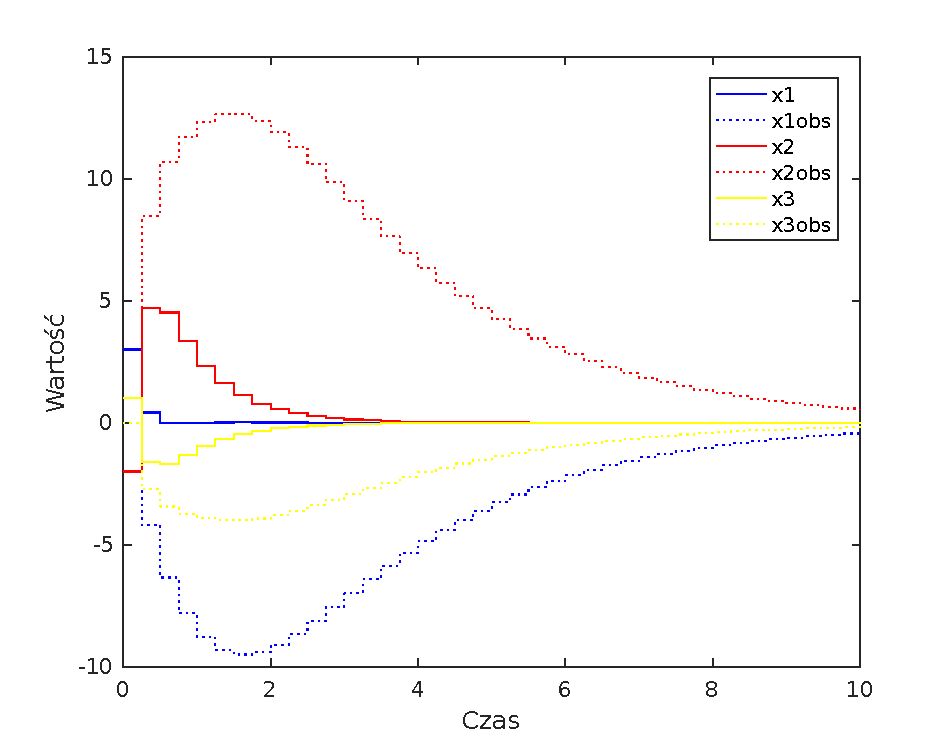
\includegraphics[width=\textwidth]{img/obs1.pdf}
\caption{Wolny obserwator $z_{o1}=0,6$, $z_{o2}=0,9$ i $z_{o3}=0,7$}
\end{figure}

\begin{figure}[H]
\centering
 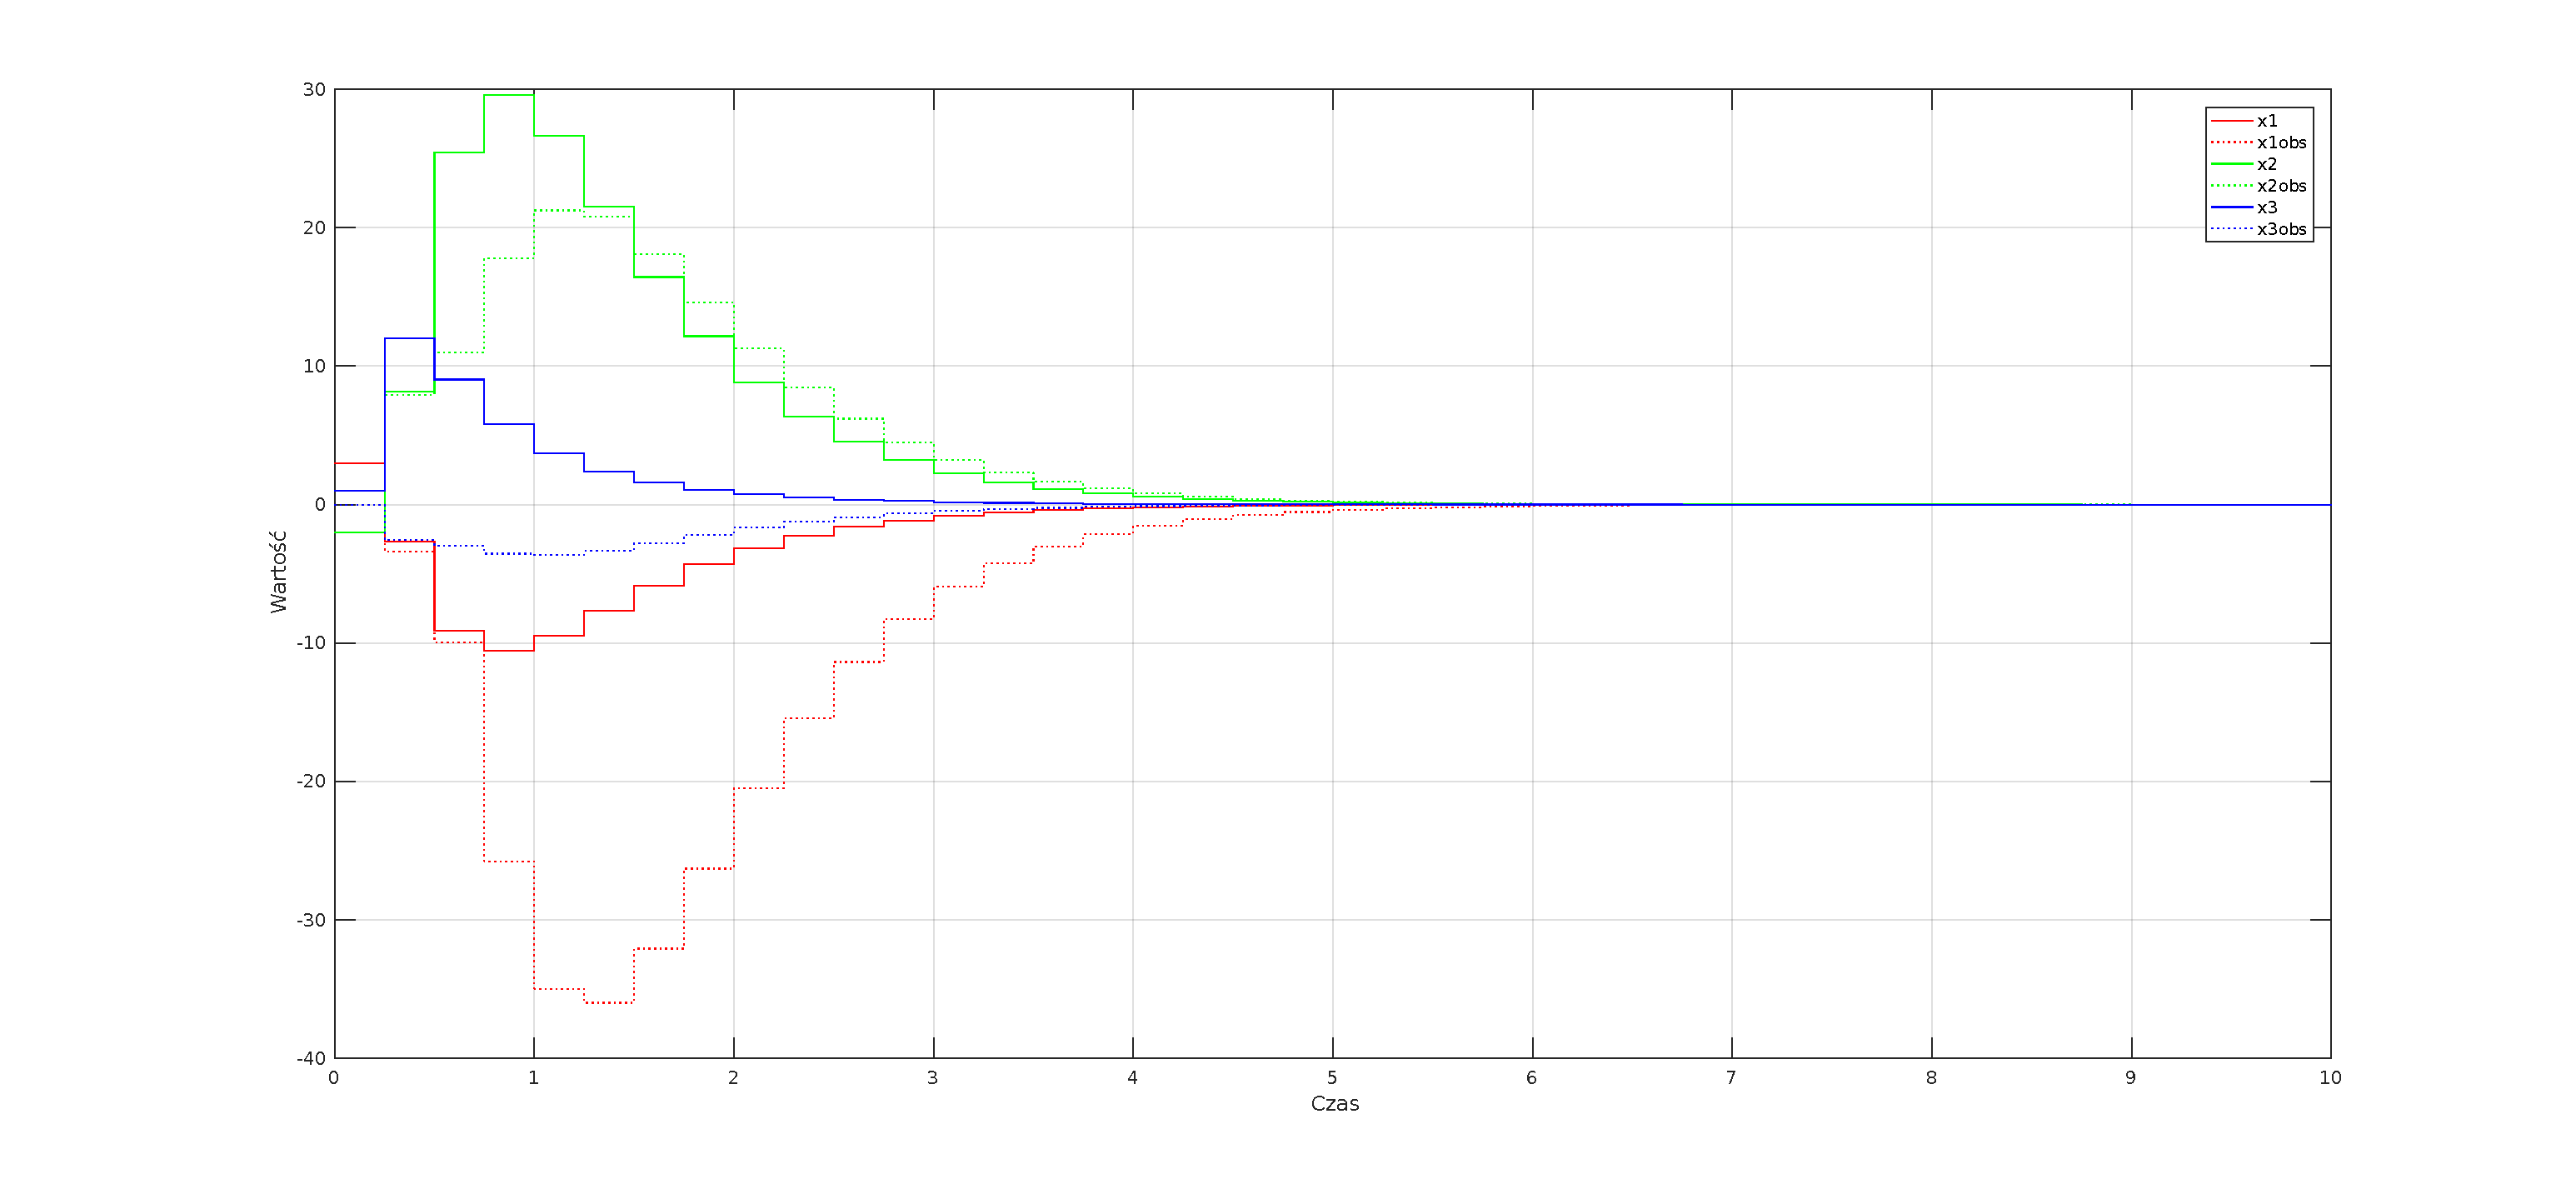
\includegraphics[width=\textwidth]{img/obs2.pdf}
\caption{Szybki obserwator $z_{o1}=0,3$, $z_{o2}=0,2$ i $z_{o3}=0,4$}
\end{figure}

Ponieważ obserwator jest jedynie programem komputerowym bez elementów wykonawczych, możemy zastosować najszybsze, zerowe bieguny.

\begin{figure}[H]
\centering
 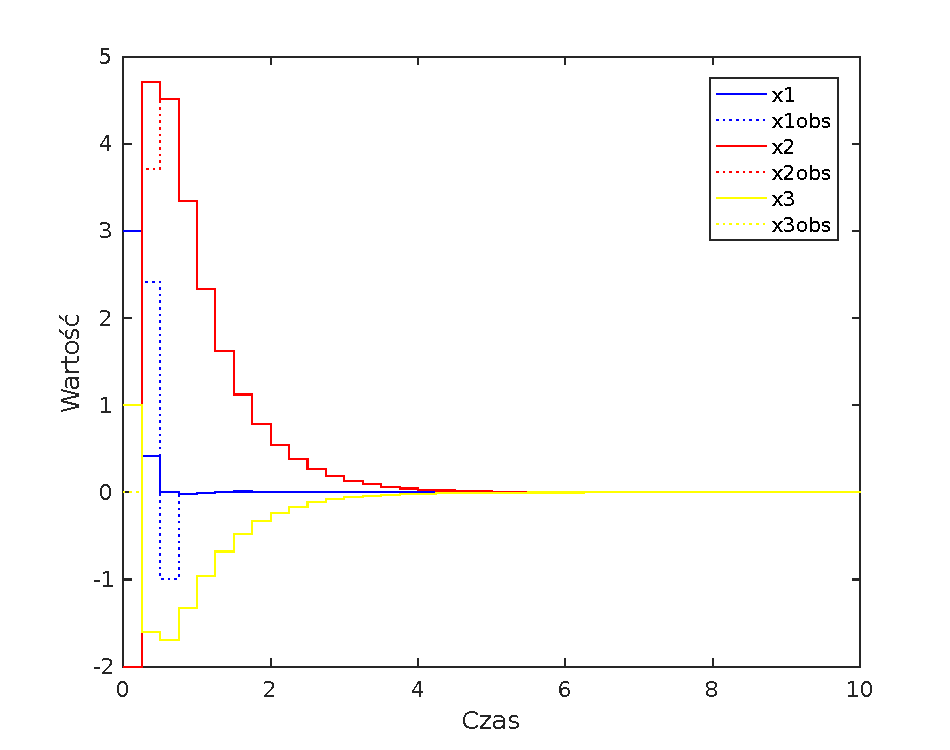
\includegraphics[width=\textwidth]{img/obs3.pdf}
\caption{Najszybszy obserwator $z_{o1}=z_{o2}=z_{o3}=0$}
\end{figure}